\documentclass[11pt,a4paper]{article}
\usepackage{fontspec}
\setmainfont{TeX Gyre Pagella}
\newfontfamily\headfont{Inter}[UprightFont=*-ExtraBold,BoldFont=*-ExtraBold,Extension=.otf,Path=/usr/share/fonts/opentype/inter/]
\usepackage[a4paper,margin=2.3cm]{geometry}
\usepackage{graphicx,booktabs,float,caption,array,xcolor,longtable}
\usepackage{xurl}
\usepackage[hidelinks]{hyperref}
\usepackage{titlesec}
\usepackage[round]{natbib}
\usepackage{setspace}
\setstretch{1.05}
\renewcommand{\topfraction}{0.9}
\renewcommand{\bottomfraction}{0.8}
\renewcommand{\textfraction}{0.1}
\renewcommand{\floatpagefraction}{0.75}
\setlength{\parindent}{0pt}
\setlength{\parskip}{0.55em}
\titleformat{\section}{\headfont\Large}{\thesection}{0.8em}{}
\titleformat{\subsection}{\headfont\large}{\thesubsection}{0.8em}{}
\captionsetup{font=small,labelfont=bf}
\urlstyle{same}
\hypersetup{pdftitle={Who named Antarctica?},pdfauthor={Tristan Hotham}}

\begin{document}
\begin{center}
{\Large\bfseries Who named Antarctica?\par}
\vspace{0.4em}
{\large The nations, years and people behind twenty thousand\\Antarctic place names\par}
\vspace{1.2em}
{\large Tristan Hotham\par}
\vspace{0.3em}
{\small Independent researcher\\
ORCID: 0000-0003-4931-9349\\
DOI: https://doi.org/10.5281/zenodo.24075309\par}
\vspace{0.8em}
2026
\end{center}

\begin{quote}
\small
\begin{center}\textbf{Abstract}\end{center}
Antarctica is the only continent whose place names were given almost entirely in the last two centuries, by many nations at once and without any resident population. Using the SCAR Composite Gazetteer of Antarctica, which combines the national gazetteers of 25 countries (39,187 names), I identify 20,151 distinct features and read each feature's narrative with documented rules to find who named it, when, and after what, linking the people honoured to Wikidata for their birthplaces. The United States named 26.1\% of features and the United Kingdom 19.8\%. Of features whose narrative records what the name means, 57.2\% honour a person and 18.2\% are descriptive, but nations differ sharply: 82.8\% of American names honour a person, 86.0\% of Japanese names are descriptive and 57.0\% of Bulgarian names recall places in Bulgaria. Claimant states name mostly inside their own claims, yet name only a minority of what they claim; the United States, which claims nothing, named 48.0\% of the features in the Ross Dependency. 43.5\% of dated names were given between 1960 and 1979. Women are 3.4\% of the people honoured; before 1990, 63.5\% of them were royals or relatives of explorers and patrons. Of the 1,449 honoured people with a known birthplace in Wikidata, 74.0\% were born in Europe. I describe the rules, their audited error rate and the limits of the narratives, and publish the feature table and an interactive map.

\textbf{Keywords:} Antarctica; toponymy; place names; gazetteer; commemoration; territorial claims; Antarctic Treaty; Wikidata; open data
\end{quote}

\section{Introduction}
Place names on other continents are layered over millennia; most of Antarctica's were given within living memory, by people who did not live there. Sealers and naval expeditions named the first coasts and islands in the 1820s to 1840s; national expeditions of the heroic age (1897 to 1922) named more; and from the 1940s aerial photography and the stations built for the International Geophysical Year (IGY, 1957 to 1958) revealed tens of thousands of mountains, glaciers and nunataks that needed names. National committees in the United States, the United Kingdom, Australia, New Zealand and elsewhere were set up to approve them \citep{alberts,stewart}.

Naming has been part of the politics of the continent. Seven states maintain territorial claims, frozen but not abandoned under Article~IV of the Antarctic Treaty \citep{treaty}, and naming a place has long been one way of asserting a presence. Because each country keeps its own gazetteer, the same feature can carry different names in different national lists. The Scientific Committee on Antarctic Research (SCAR) brings the national lists together in a Composite Gazetteer of Antarctica \citep{scar}, linking the names of the same feature with a common identifier.

This paper uses that gazetteer to ask a simple set of questions at the scale of the whole continent. Which nations named Antarctica, and where? When were the names given? What are they named after, and whom? And where were the honoured people born?

\section{Data}
\subsection{The SCAR Composite Gazetteer}
The gazetteer extract, from the Australian Antarctic Data Centre, holds 39,187 names in 25 national gazetteers and a list of undersea features (Table~\ref{tab:gaz}). Each record gives the name, the country whose gazetteer lists it, coordinates, feature type, a common identifier shared by the names of the same feature in other gazetteers, approval dates where recorded, and usually a narrative describing the feature and how it was named. Some gazetteers (Germany, Australia, New Zealand) also have a separate ``named for'' field. The gazetteer is released under CC BY 4.0.

\begin{table}[tbp]\centering\small\caption{Names in each national gazetteer of the SCAR Composite Gazetteer, and features listed only there (the sixteen largest lists).}\label{tab:gaz}\begin{tabular}{lrr}\toprule Gazetteer & Names & Only in this list\\\midrule
United States & 13,192 & 1,918\\
United Kingdom & 5,181 & 457\\
Russia & 4,808 & 963\\
New Zealand & 3,577 & 243\\
Australia & 2,587 & 484\\
Argentina & 2,560 & 393\\
Chile & 1,866 & 281\\
Norway & 1,706 & 579\\
Bulgaria & 1,540 & 1,470\\
Germany & 399 & 275\\
Poland & 365 & 292\\
China & 364 & 319\\
Japan & 345 & 181\\
France & 227 & 127\\
Undersea (SCUFN) & 182 & 80\\
Belgium & 117 & 4\\
\bottomrule\end{tabular}\end{table}

Grouping the records by common identifier gives 20,151 features, after merging 8 pairs of identifiers that hold the same name within five kilometres (documented in \texttt{data/overrides\_merge.csv}). 11,945 features (59.3\%) appear in more than one national gazetteer.

\subsection{Wikidata}
A Wikidata \citep{wikidata} extract, queried through QLever \citep{qlever}, gives features with coordinates in Antarctica, what they are ``named after'' (property P138) and, for people, their place and date of birth. Wikidata features were matched to gazetteer features by name within 25~km: 17,028 of 19,693 (86.5\%). 1,998 gazetteer features are thereby linked to 1,772 people, 1,449 of them with a located birthplace. Birthplaces were placed in modern countries and continents with Natural Earth \citep{naturalearth}. The base map uses OpenStreetMap \citep{osm} coastlines, which include the ice shelves, and Natural Earth land, which does not.

\section{Methods}
\subsection{Reading the narratives}
Rules written in Python (published as \texttt{code/parse.py}) read each narrative. The \emph{naming statement} is the first sentence with the word ``named'' followed by ``for'', ``after'', ``in honour of'', ``because'' or ``in association with''; Norwegian entries beginning ``After'', Spanish and French equivalents, and translations given in brackets (``named Mikazuki Iwa (crescent rock)'') are also read. The words between ``named'' and the preposition (``by US-ACAN'', ``by the BrAE'', ``by Charcot'') are matched to a list of committees, expeditions and leaders, each assigned to a nation. The text after the preposition, the \emph{honoree clause}, is classified by its opening words into a person, a group of people, a ship, an aircraft or vehicle, an institution or operation, a place elsewhere, an event, myth and fiction, a star, letter, word or work, wildlife and plants, a description, a nearby feature (association), or other.

For each feature the naming nation is taken from the first narrative that names a namer, in a fixed order of gazetteers (United States, United Kingdom, New Zealand, Australia, then others). Where none does, it is the only national gazetteer holding the feature (ignoring the Russian list where one other list holds it, because the Russian list transliterates most other nations' names), then the expedition the narrative says discovered or charted the feature, then the gazetteer with the earliest approval date. Table~\ref{tab:src} shows how many features each rule decides. The naming year is the earliest year in a naming statement (excluding life dates) or an approval citation, and otherwise the first approval date in any gazetteer.

\subsection{People, roles and women}
For features named after a person, the honoree's name and surname are extracted after removing titles and ranks. What the person did is read from the clause by keyword, in priority order: royalty, heads of state and politicians; patrons, sponsors and officials; scientists and surveyors; naval and military personnel; support staff; explorers, whalers and sealers; writers, artists and composers. Every feature whose honoree clause suggests a woman was read by hand: a female title or relative, ``she'' or ``her'', a female given name (from a list and from the \texttt{gender-guesser} name dictionary), a Slavic feminine surname, or a namesake whose Wikidata sex (P21) is female. That gives 368 candidates, 315 confirmed (\texttt{data/overrides\_women.csv}); 106 of these were found in an independent review of the first pass. The rejections were mostly men named Jean, Marion or Leslie and ships referred to as ``her''. Features named after a couple or a family are not counted as honouring a woman.

\subsection{Checks}
Data errors of three kinds were looked for across the whole set. Duplicates: features with the same name within five kilometres under different identifiers (8 merged). Wikidata links: every link whose namesake's name does not appear in the feature's names was read; most were transliterations or alternative names; 5 wrong links (for example Plata Passage, named after the River Plate estuary, linked to a Chilean admiral) were removed. Birthplaces given only as a country or state, found by searching for round coordinates and birthplace items that are countries: 21 are left off the map (\texttt{data/overrides\_people.csv}). The rule-based reading was audited twice on random samples. A first audit of 100 features, before the rules were refined, found about one in ten misread. A second audit of 60 features (58 decidable) found 7 misreadings, 93.1\% correct (\texttt{data/audit\_sample\_60.csv}); most errors put a person into ``other'' or ``not stated''. Finally the naming nation of every land, coast, sea and ice shelf (153 features) was read by eye and 7 were corrected, together with 214 documented corrections in all (\texttt{data/overrides\_features.csv}). Of these, 196 come from an independent review that reread the ``other'' class, every feature linked to a Wikidata person but not classed as one, and the features classed as people whose narrative is a Soviet descriptive name. Finally, 226 British approval dates stored in the source a century early (1901 to 1910 for UK-APC decisions of 2001 to 2010; the older date field and the narratives give the true year) were corrected.

\begin{table}[tbp]\centering\small\caption{How the naming nation was decided.}\label{tab:src}\begin{tabular}{lrr}\toprule Rule & Features & \%\\\midrule
Naming statement names the namer & 10,831 & 53.7\\
Only one national list holds it & 6,397 & 31.7\\
Expedition said to have discovered or charted it & 1,559 & 7.7\\
Earliest approval date & 956 & 4.7\\
Corrected by hand & 7 & 0.0\\
Not known & 401 & 2.0\\
\bottomrule\end{tabular}\end{table}

\section{Results}
\subsection{The naming nations}
Figure~\ref{fig:map} maps every feature by naming nation and Figure~\ref{fig:nations} counts them. The United States named 5,253 features (26.1\%) and the United Kingdom 3,981 (19.8\%), together 45.8\%. Norway, Bulgaria, Australia, New Zealand and Russia follow with between 6.4\% and 7.9\% each (Table~\ref{tab:nations}). 26 nations named at least one feature; the naming nation is unknown for 401.

\begin{figure}[tbp]\centering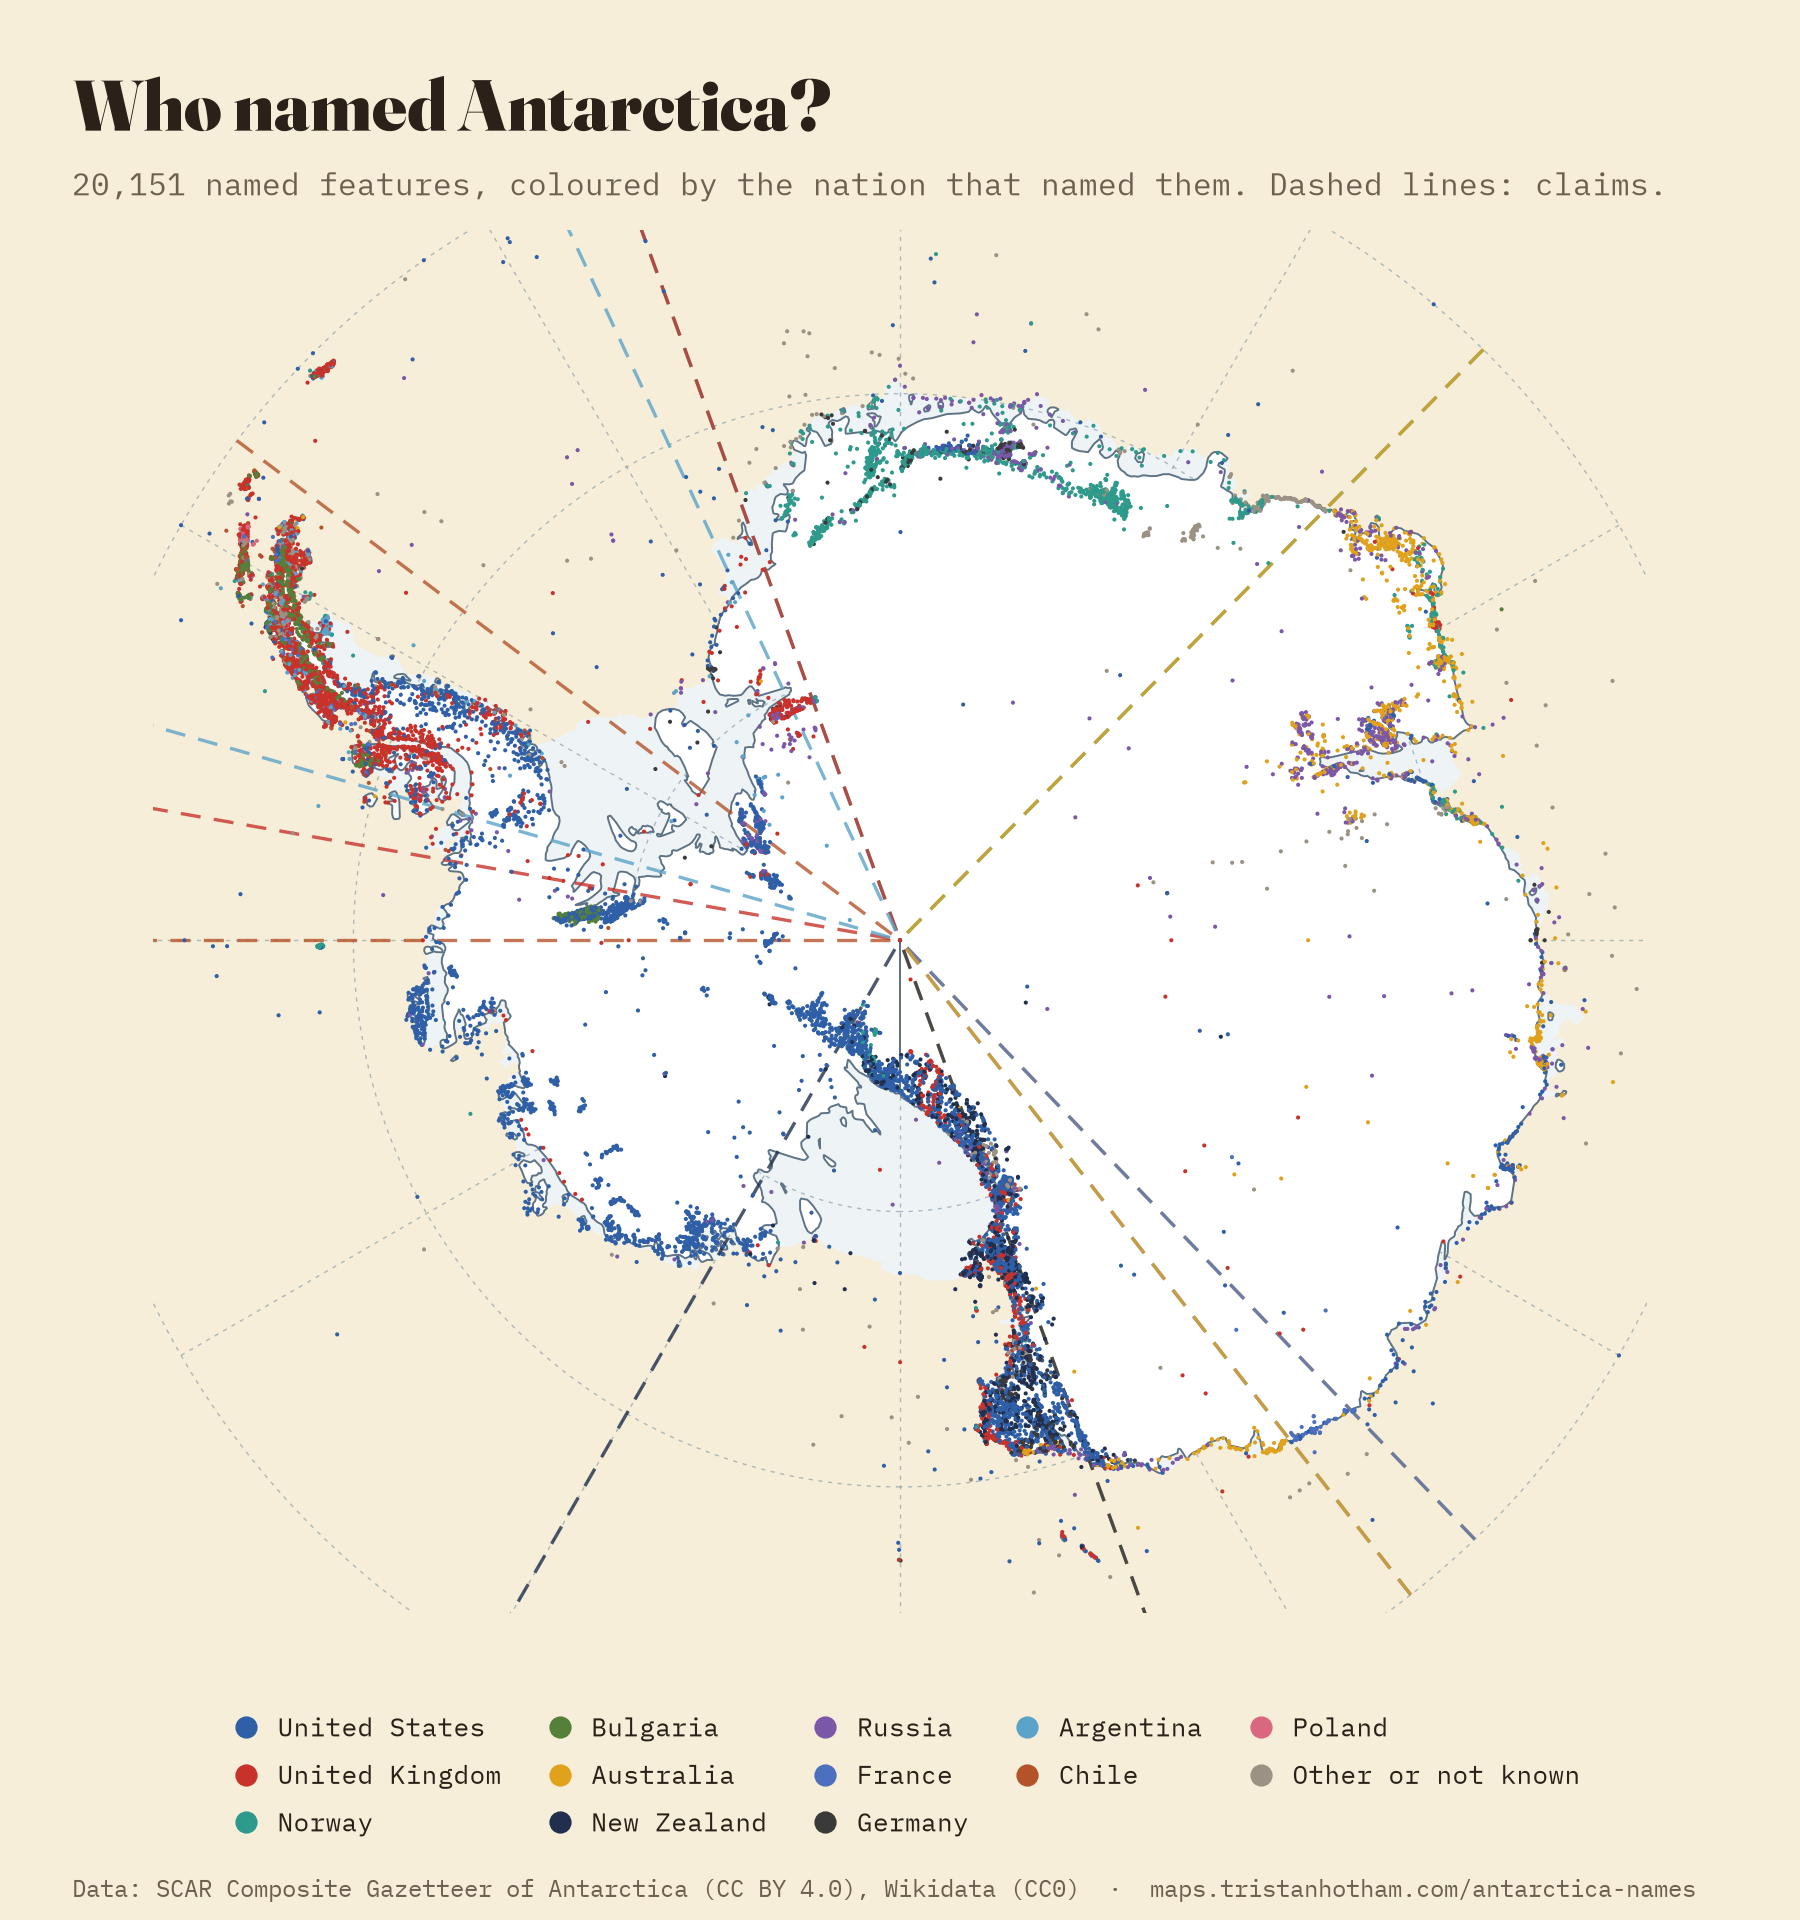
\includegraphics[width=0.92\textwidth]{f_map.png}
\caption{Every named feature in the gazetteer, coloured by naming nation, on a polar stereographic projection (EPSG:3031). Dashed lines mark the national claims.}\label{fig:map}\end{figure}
\begin{figure}[tbp]\centering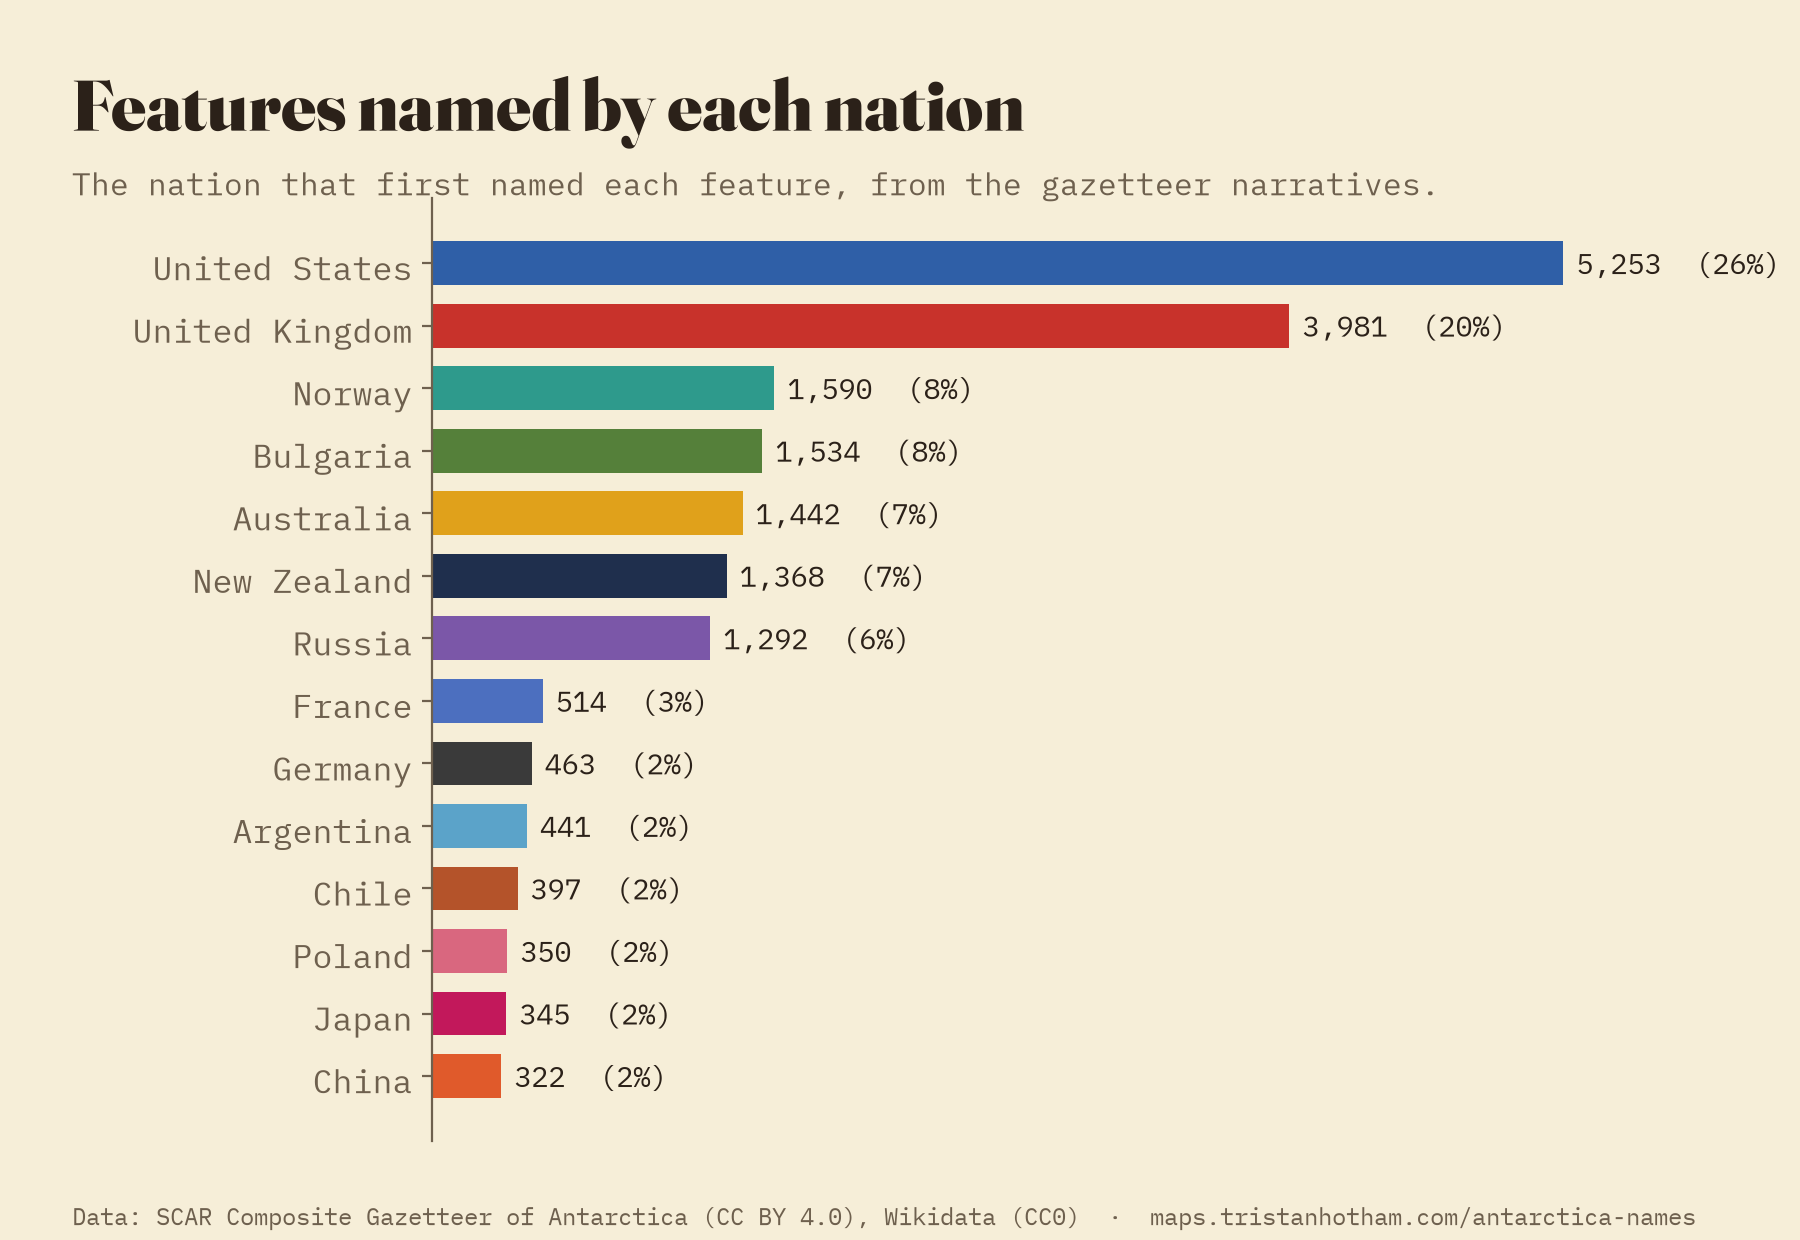
\includegraphics[width=0.85\textwidth]{f_nations.png}
\caption{Features named by each nation.}\label{fig:nations}\end{figure}

\begin{table}[tbp]\centering\small\caption{The fifteen leading naming nations: features, share of all features, shares (of features with a recorded meaning) named after a person, descriptive and after a place elsewhere, median naming year, and share of the nation's names inside its own claim.}\label{tab:nations}\begin{tabular}{lrrrrrrr}\toprule Nation & Features & \% & Person & Descr. & Place & Year & In claim\\\midrule
United States & 5,253 & 26.1 & 82.8 & 7.0 & 0.3 & 1967 & \\
United Kingdom & 3,981 & 19.8 & 52.6 & 21.9 & 0.9 & 1960 & 83.6\\
Norway & 1,590 & 7.9 & 26.9 & 60.9 & 1.4 & 1966 & 79.7\\
Bulgaria & 1,534 & 7.6 & 25.9 & 3.0 & 57.0 & 2011 & \\
Australia & 1,442 & 7.2 & 69.6 & 10.8 & 1.3 & 1965 & 95.8\\
New Zealand & 1,368 & 6.8 & 36.5 & 28.1 & 1.4 & 1965 & 84.3\\
Russia & 1,292 & 6.4 & 56.4 & 24.0 & 4.4 & 1970 & \\
France & 514 & 2.5 & 63.0 & 14.9 & 2.2 & 1952 & 39.7\\
Germany & 463 & 2.3 & 44.4 & 14.7 & 6.8 & 1985 & \\
Argentina & 441 & 2.2 & 26.5 & 10.2 & 4.1 & 1978 & 99.5\\
Chile & 397 & 2.0 & 63.5 & 10.1 & 0.6 & 1971 & 100.0\\
Poland & 350 & 1.7 & 64.8 & 1.5 & 6.1 & 1981 & \\
Japan & 345 & 1.7 & 2.9 & 86.0 & 0.0 & 1975 & \\
China & 322 & 1.6 & 4.2 & 20.8 & 4.2 & 1992 & \\
Belgium & 160 & 0.8 & 71.3 & 5.3 & 3.3 & 1955 & \\
\bottomrule\end{tabular}\end{table}

\subsection{Naming and claims}
Claimant states name mostly inside their own sectors: 99.5\% of Argentina's names, 95.8\% of Australia's, 84.3\% of New Zealand's, 83.6\% of the United Kingdom's and 79.7\% of Norway's. France is the exception (39.7\%), because Charcot's expeditions of 1903 to 1910 named much of the western Antarctic Peninsula before Ad\'elie Land was explored. Yet claimants name only part of what they claim (Figure~\ref{fig:claims}): Norway named 55.8\% of the features in Dronning Maud Land, Australia 37.9\% of those in the Australian Antarctic Territory and New Zealand 28.9\% of those in the Ross Dependency, where the United States named 48.0\%. In unclaimed Marie Byrd Land the United States named 95.7\%. In the overlapping Peninsula claims, Argentina named 5.5\% and Chile 4.9\% of the features in their own claims, while the United Kingdom named 40.8\% of those in the Argentine claim.

\begin{figure}[tbp]\centering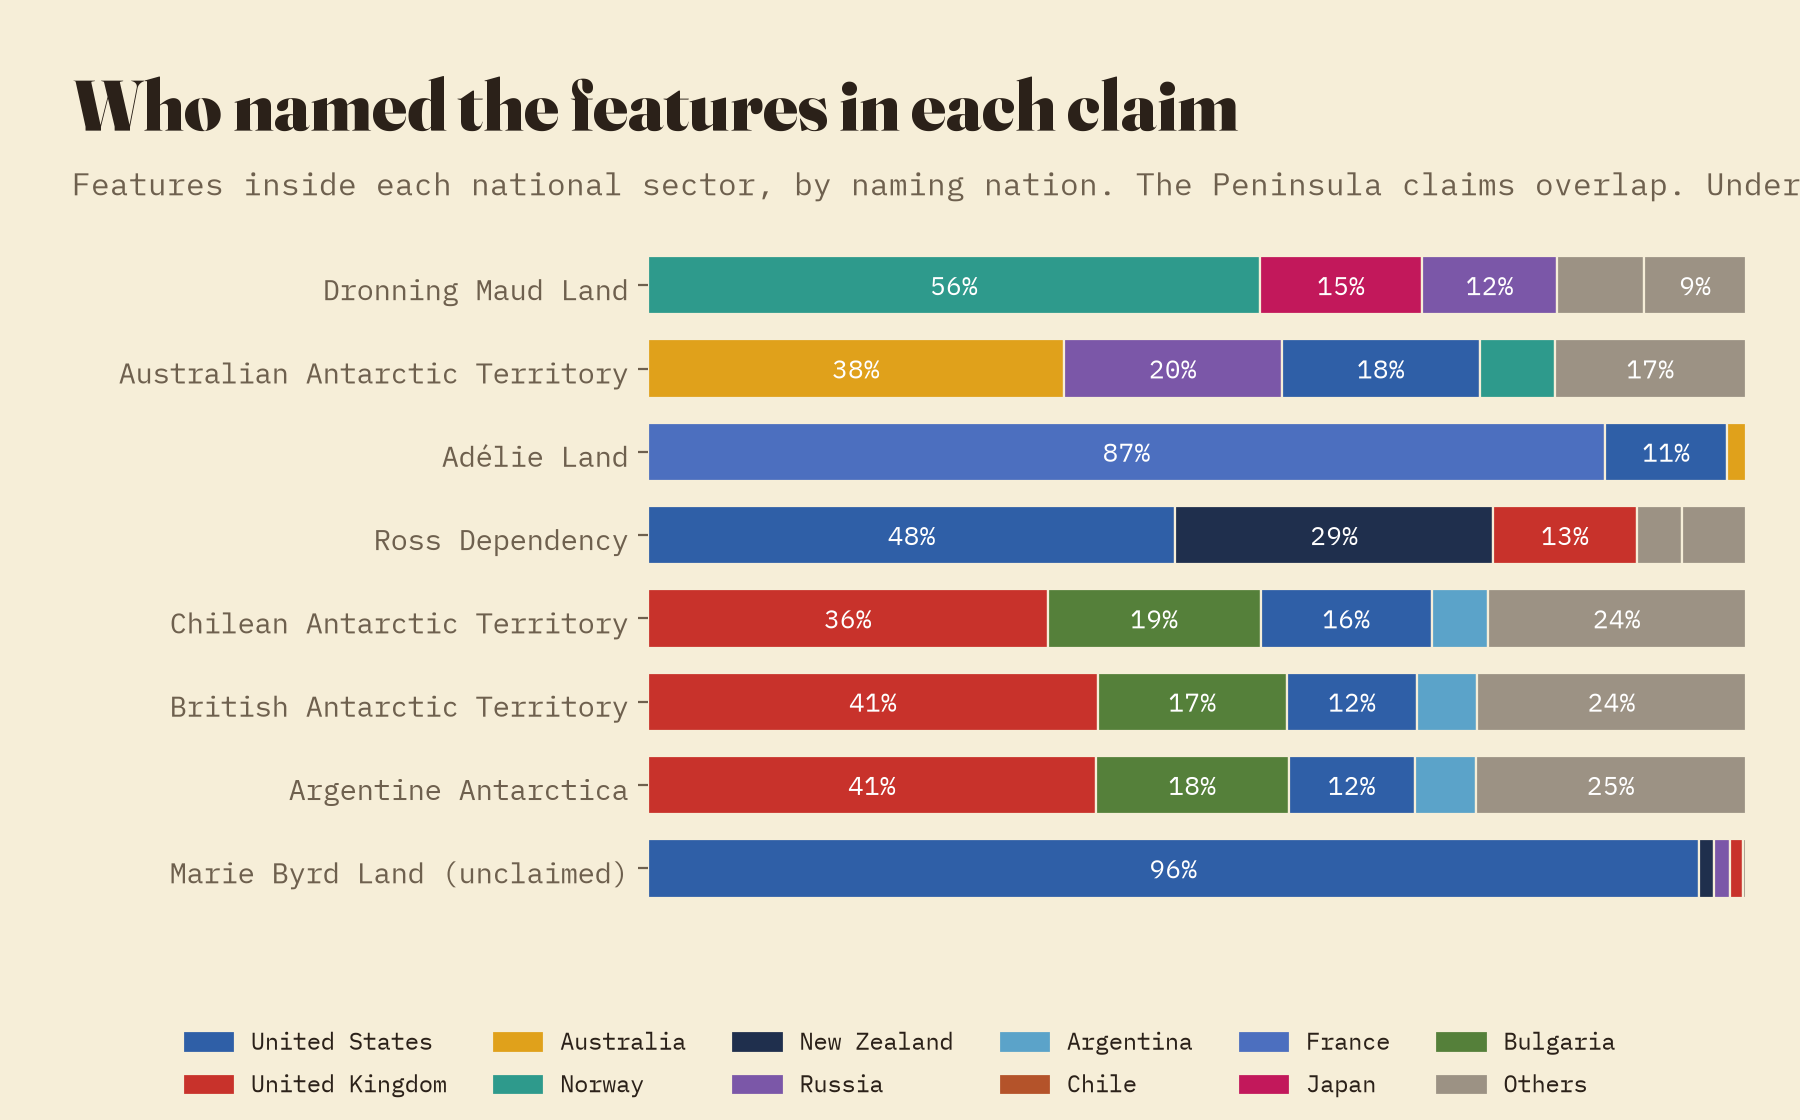
\includegraphics[width=0.9\textwidth]{f_claims.png}
\caption{Features inside each claim, by naming nation.}\label{fig:claims}\end{figure}

\subsection{When}
Figure~\ref{fig:decades} shows names by decade. Only 98 dated names carry a date before 1900 and 148 a date in the heroic age, although many more were given in those years and are dated here by a later approval. The post-war surveys and the IGY brought the great wave: 2,743 names from 1946 to 1956, 991 in 1957 to 1959 and 7,472 (43.5\%) from 1960 to 1979, with a peak of 5,384 in the 1960s, nearly half of them American names for features photographed by US Navy aircraft. Naming continues: 3,105 names (18.1\%) date from 2000 or later, 48.0\% of them Bulgarian. Because the naming year is often an approval date, the profile is shifted later than first use; Table~\ref{tab:eras} gives the counts by period.

\begin{figure}[tbp]\centering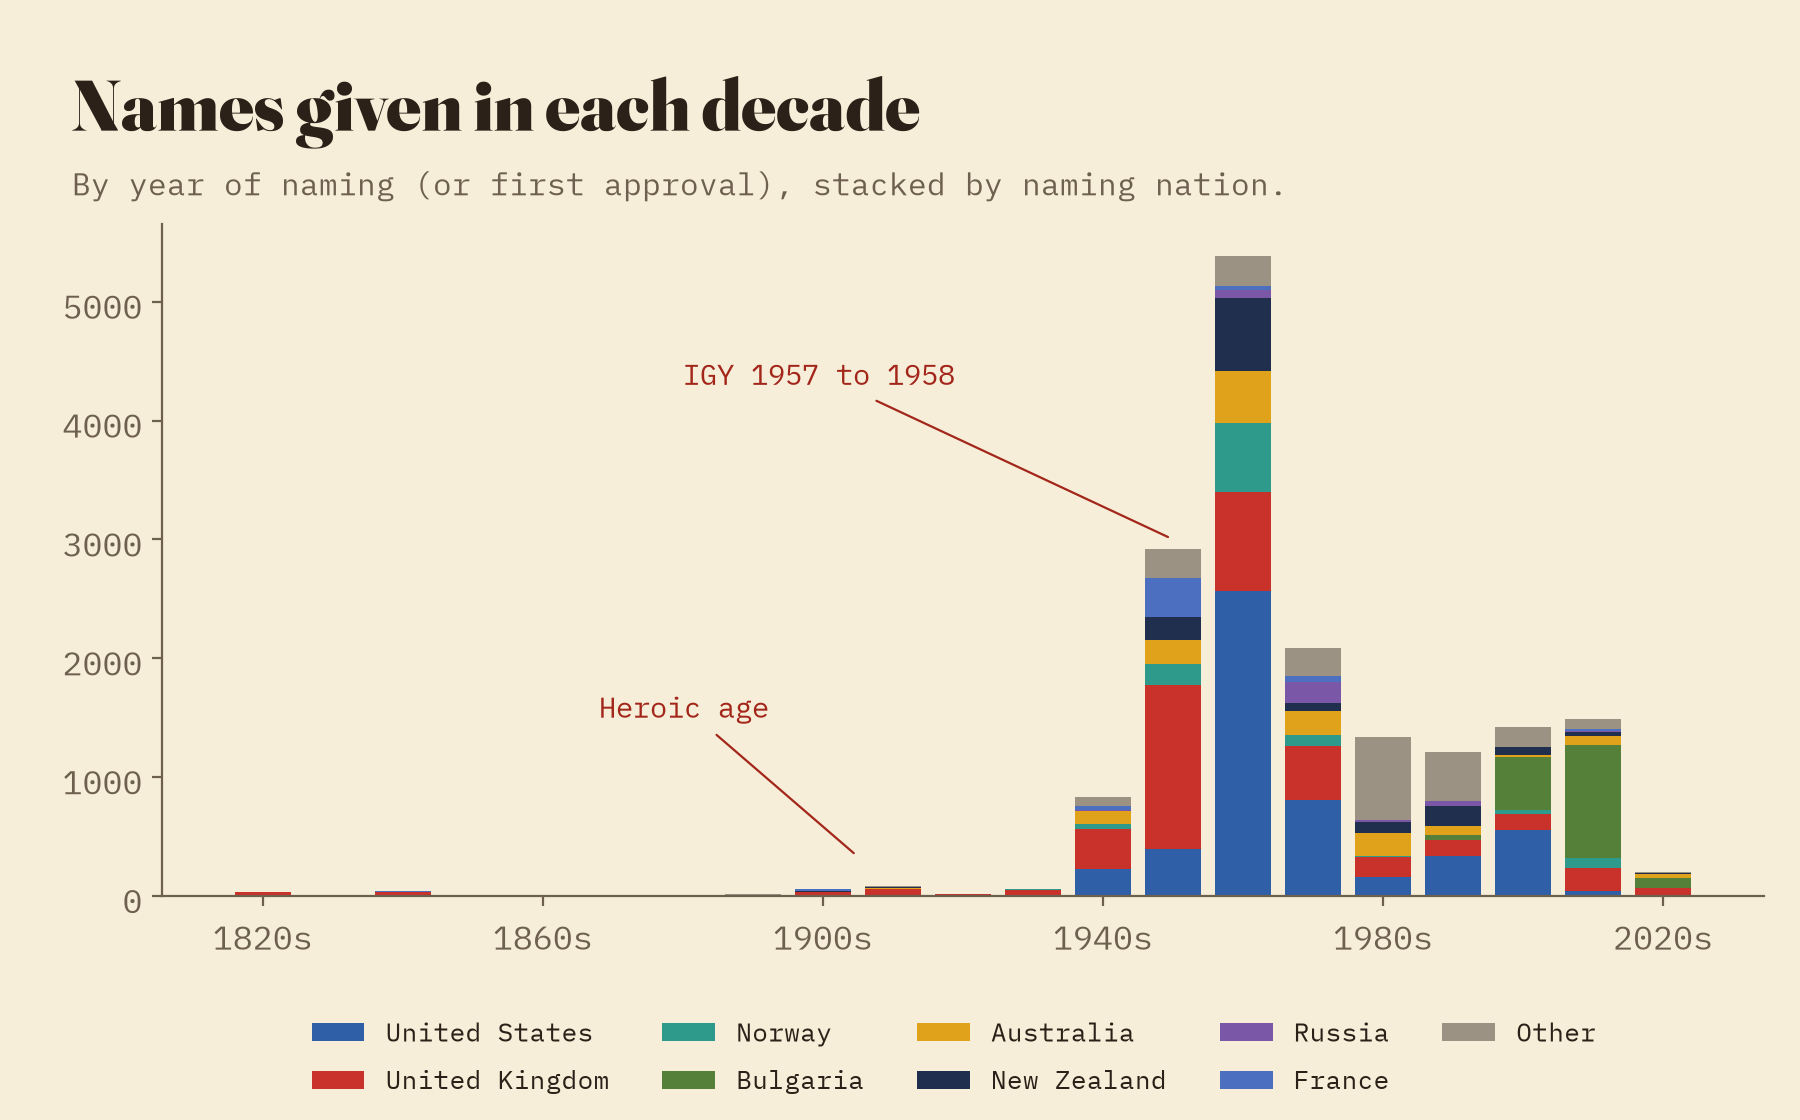
\includegraphics[width=0.9\textwidth]{f_decades.png}
\caption{Features by decade of naming, stacked by naming nation.}\label{fig:decades}\end{figure}

\begin{table}[tbp]\centering\small\caption{Dated features by period of naming, with the three leading naming nations.}\label{tab:eras}\begin{tabular}{lrrl}\toprule Period & Features & \% & Leading nations\\\midrule
Before 1897 & 92 & 0.5 & United Kingdom, France, United States\\
Heroic age, 1897 to 1922 & 148 & 0.9 & United Kingdom, France, New Zealand\\
1923 to 1945 & 94 & 0.6 & United Kingdom, United States, Australia\\
1946 to 1956 & 2,743 & 15.9 & United Kingdom, United States, France\\
IGY, 1957 to 1959 & 991 & 5.8 & United Kingdom, New Zealand, Australia\\
1960 to 1979 & 7,472 & 43.5 & United States, United Kingdom, Norway\\
1980 to 1999 & 2,549 & 14.8 & United States, Poland, United Kingdom\\
2000 onwards & 3,105 & 18.1 & Bulgaria, United States, United Kingdom\\
\bottomrule\end{tabular}\end{table}

\subsection{What the names honour}
For 16,354 features (81.2\%) the narrative records what the name means. 57.2\% honour a person, 18.2\% describe the feature, 6.3\% recall a place elsewhere, 4.7\% take the name of a nearby feature and 2.6\% honour a ship. The national styles differ (Figure~\ref{fig:kinds}): 82.8\% of American names honour a person against 26.9\% of Norwegian ones; 60.9\% of Norwegian and 86.0\% of Japanese names are descriptive; 57.0\% of Bulgarian names recall places in Bulgaria, one of the clearest uses of Antarctic naming to project a national geography.

\begin{figure}[tbp]\centering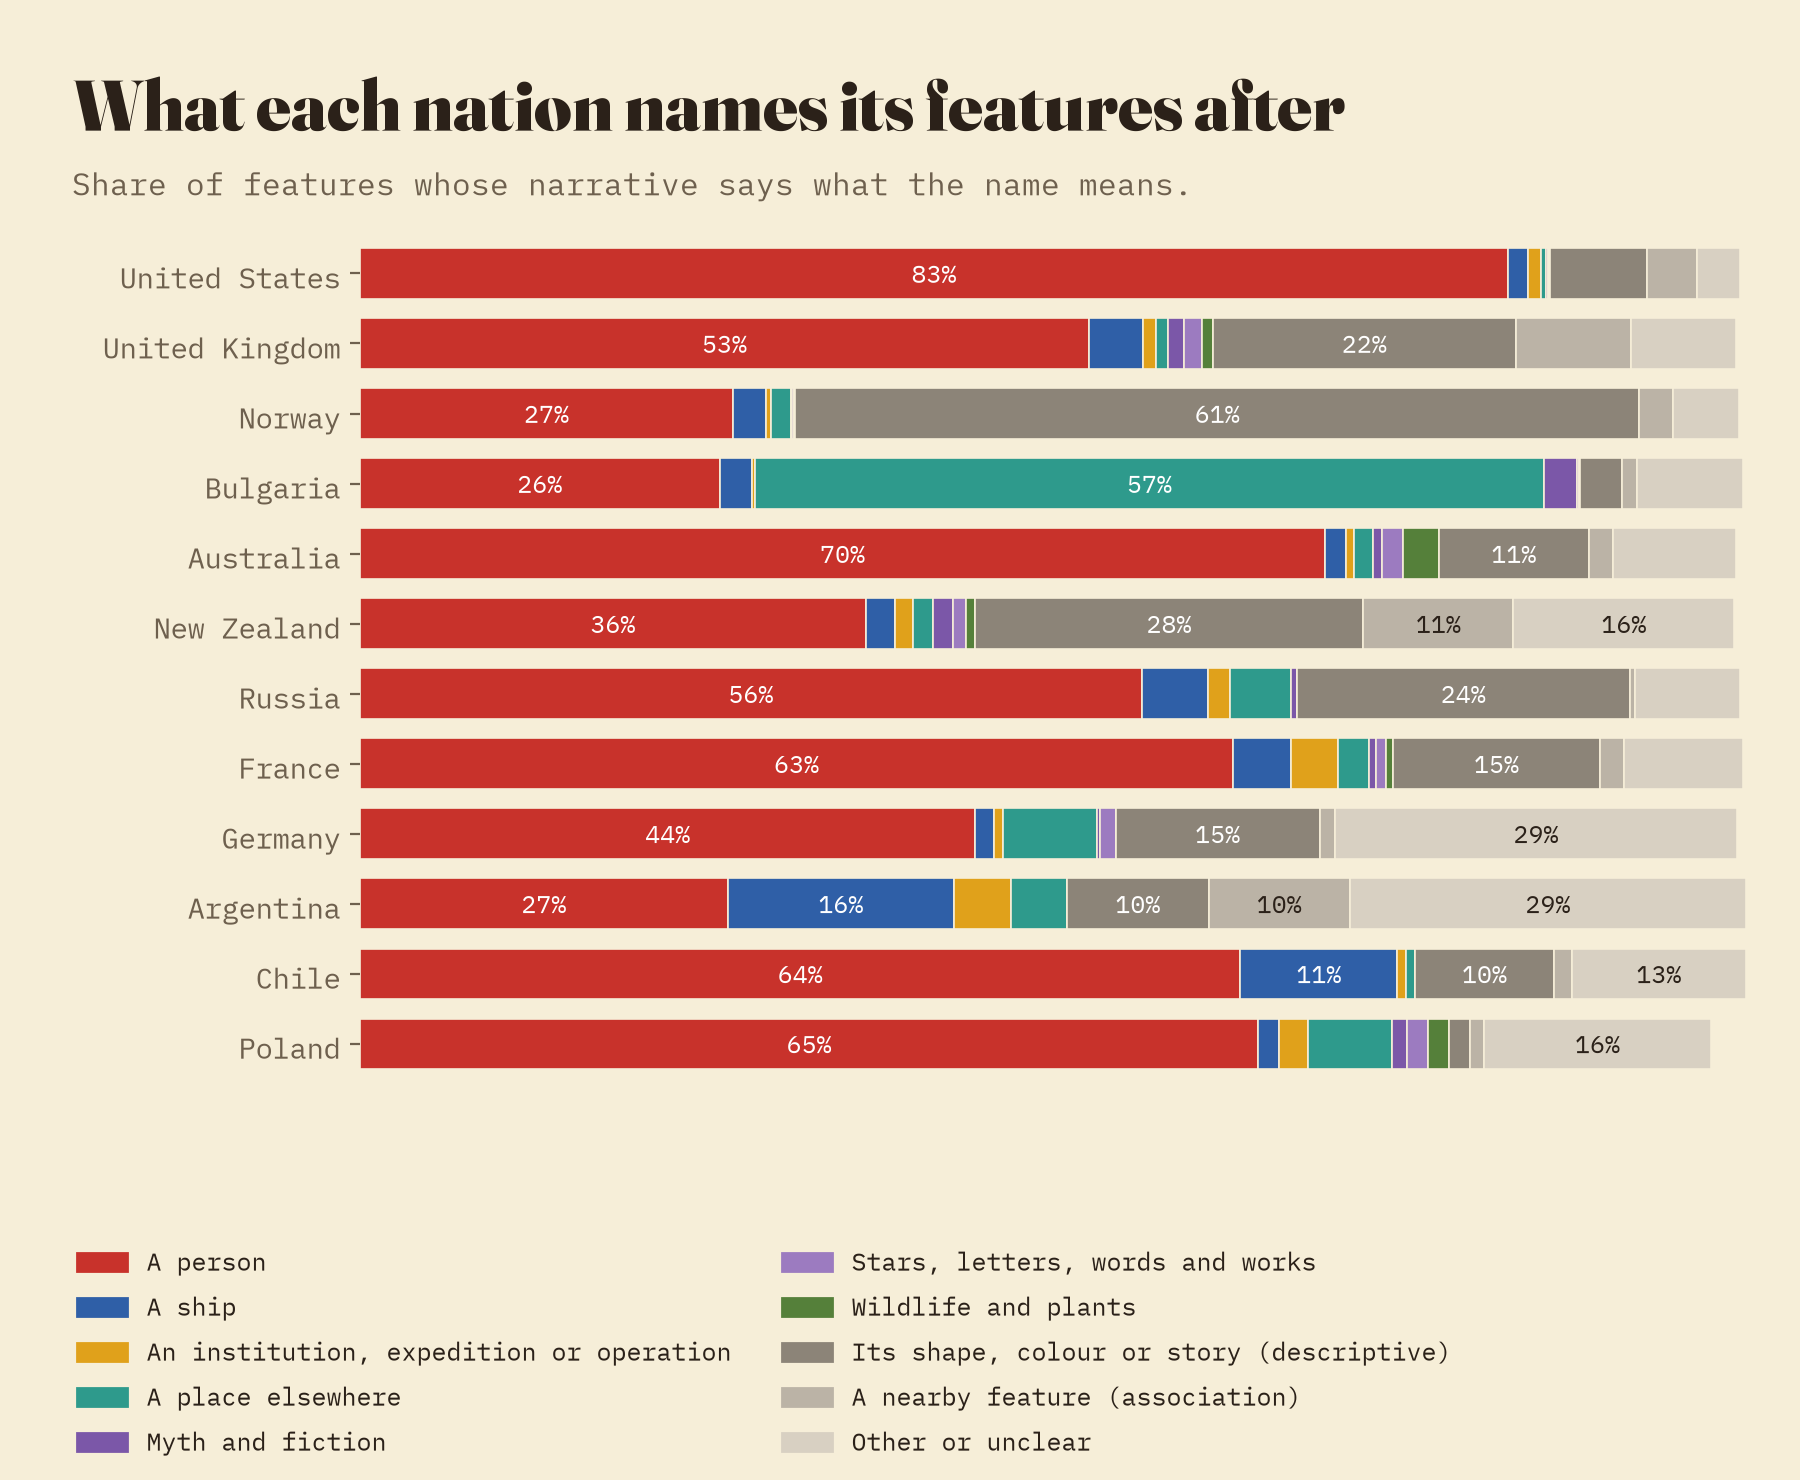
\includegraphics[width=0.9\textwidth]{f_kinds.png}
\caption{What each nation's features are named after, among features whose narrative records it.}\label{fig:kinds}\end{figure}

\subsection{Who is honoured}
The commonest surnames among features named after a person are Smith (35), Davis (23), Brown (22), Johnson (21) and Wilson (19): the map honours many ordinary members of national programmes. Read by keyword (Figure~\ref{fig:roles}), 33.4\% of the people were scientists or surveyors, 18.2\% naval or military personnel, 8.5\% support staff and 5.3\% royalty, heads of state or politicians. 30.4\% of the people on American names were naval or military, reflecting the US Navy's role in Operation Deep Freeze; 24.7\% of those on Australian names were station staff such as cooks and radio officers; 18.0\% of those on Bulgarian names are rulers or politicians of Bulgarian history.

\begin{figure}[tbp]\centering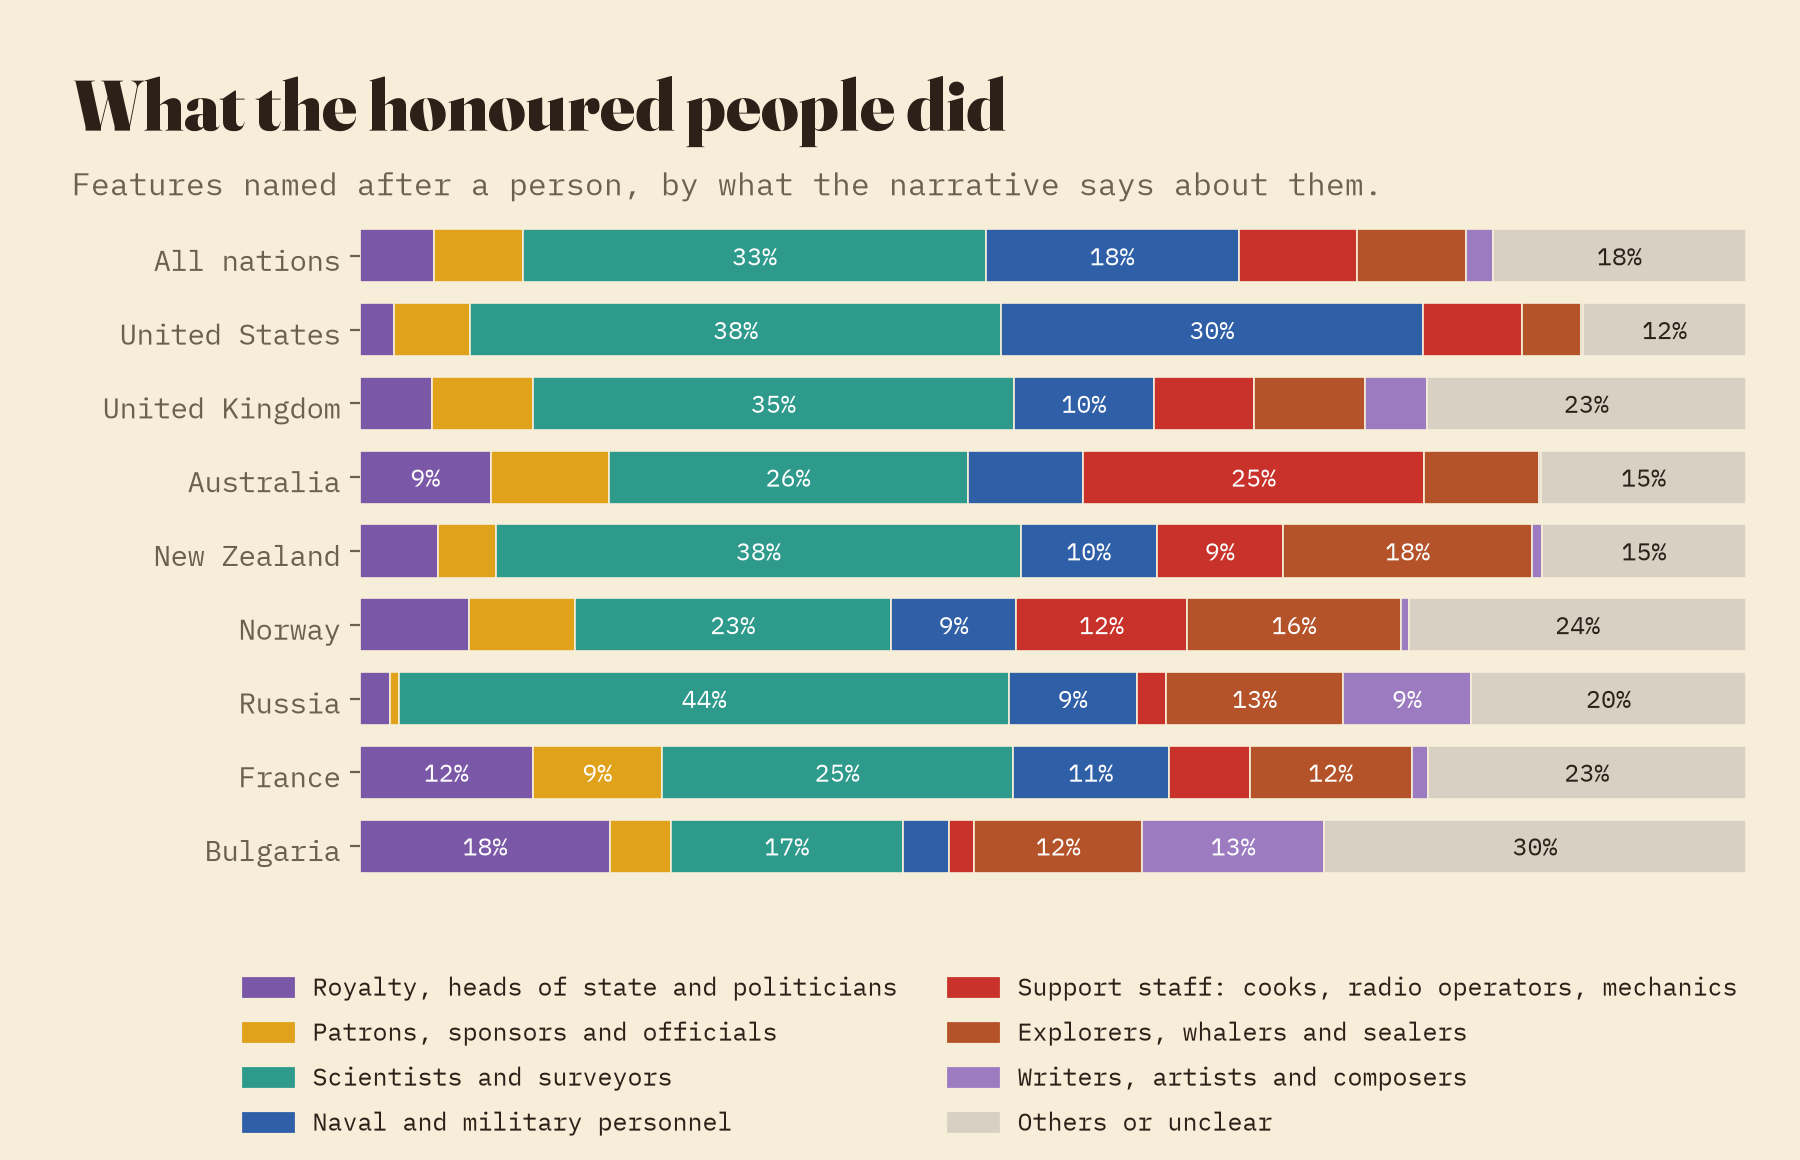
\includegraphics[width=0.9\textwidth]{f_roles.png}
\caption{What the people honoured did, read from the narratives, by naming nation.}\label{fig:roles}\end{figure}

\subsection{Women}
315 of 9,353 features named after a person honour a woman (3.4\%). They include some of the largest names on the map, such as Queen Maud Land, Victoria Land and Marie Byrd Land. Before 1990, 63.5\% of the women honoured were royals or the wives, daughters, mothers and sisters of explorers and patrons; since 1990 the share of women among the people honoured has risen from 1.9\% to 10.3\%, and only 6.3\% of them are honoured as relatives or royals (Figure~\ref{fig:women}). The share was lowest from 1960 to 1979 (1.0\%), the years of the naval air operations.

\begin{figure}[tbp]\centering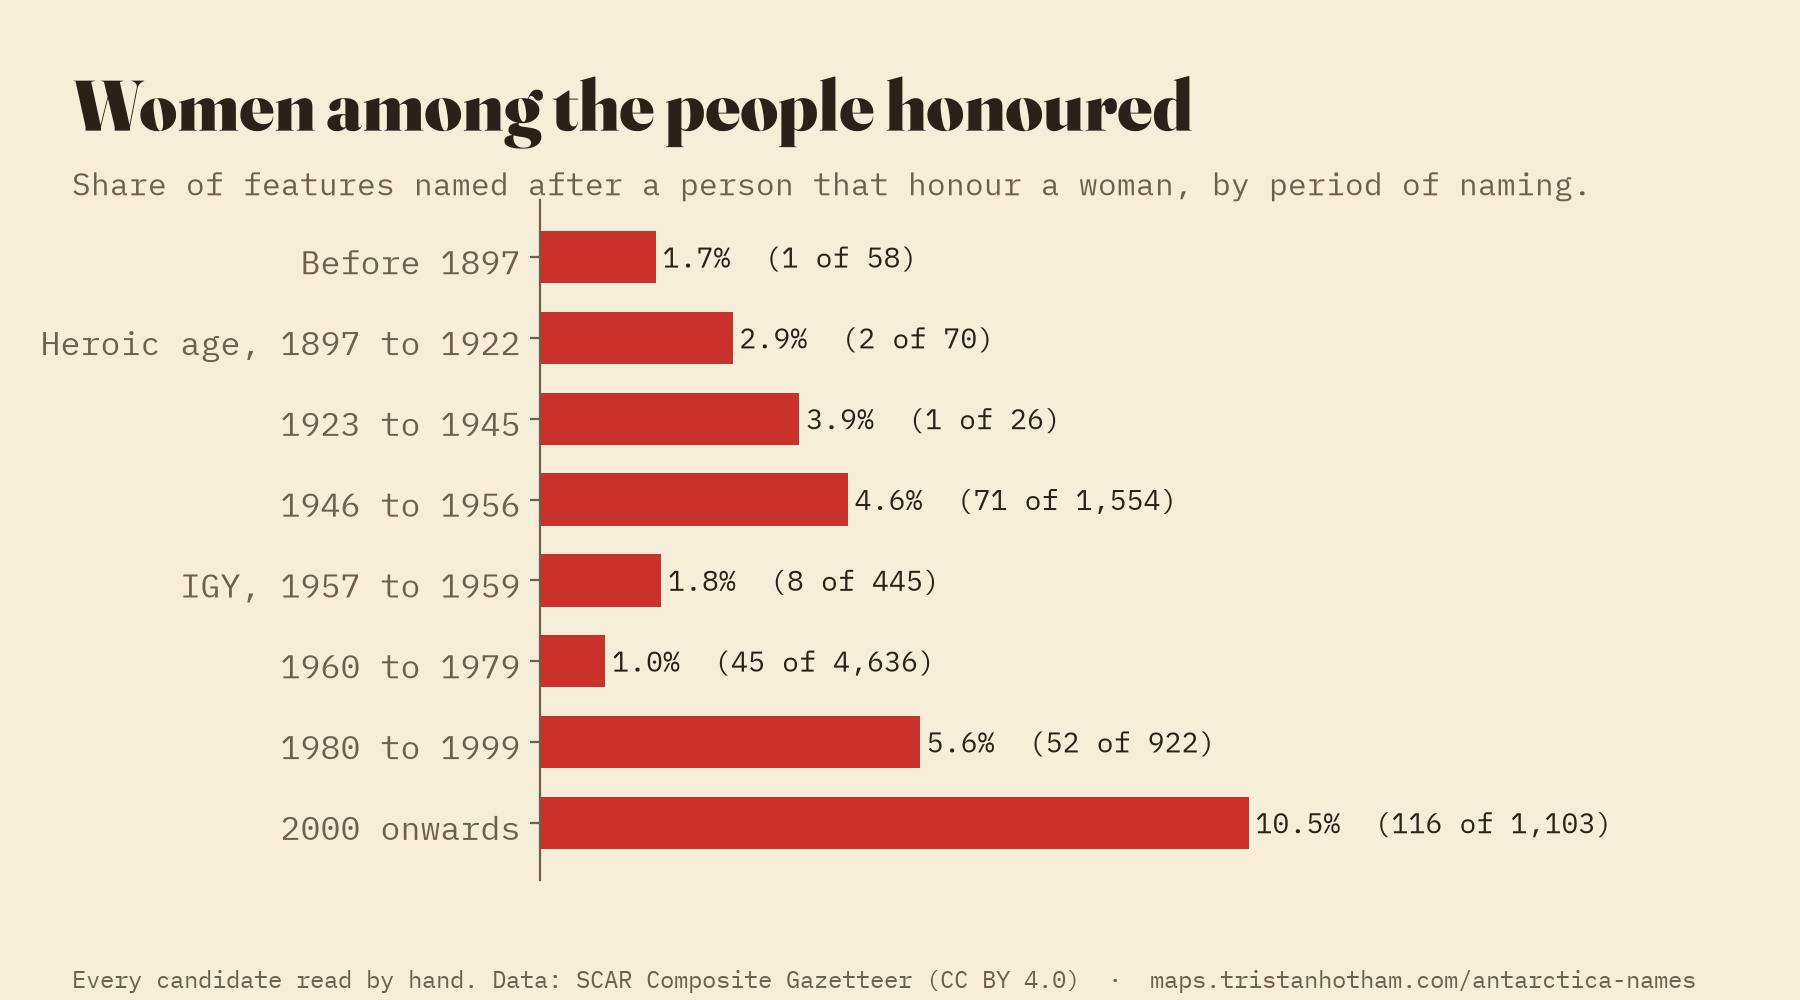
\includegraphics[width=0.85\textwidth]{f_women.png}
\caption{Women among the people honoured, by period of naming.}\label{fig:women}\end{figure}

\subsection{Where the honoured were born}
Of 1,449 people with a located birthplace (Figure~\ref{fig:birth}), 74.0\% were born in Europe and 17.5\% in North America; Oceania has 66, Asia 33, South America 18 and Africa 7. The United Kingdom (307), the United States (239), France (166) and Norway (132) lead. Nations differ in how far they look: 81.0\% of the people on Norwegian names were born in Norway and 57.9\% of those on American names in the United States, against 40.2\% for British names (which honour many foreign scientists, for example in themed groups of names) and 33.3\% for Australian names.

\begin{figure}[tbp]\centering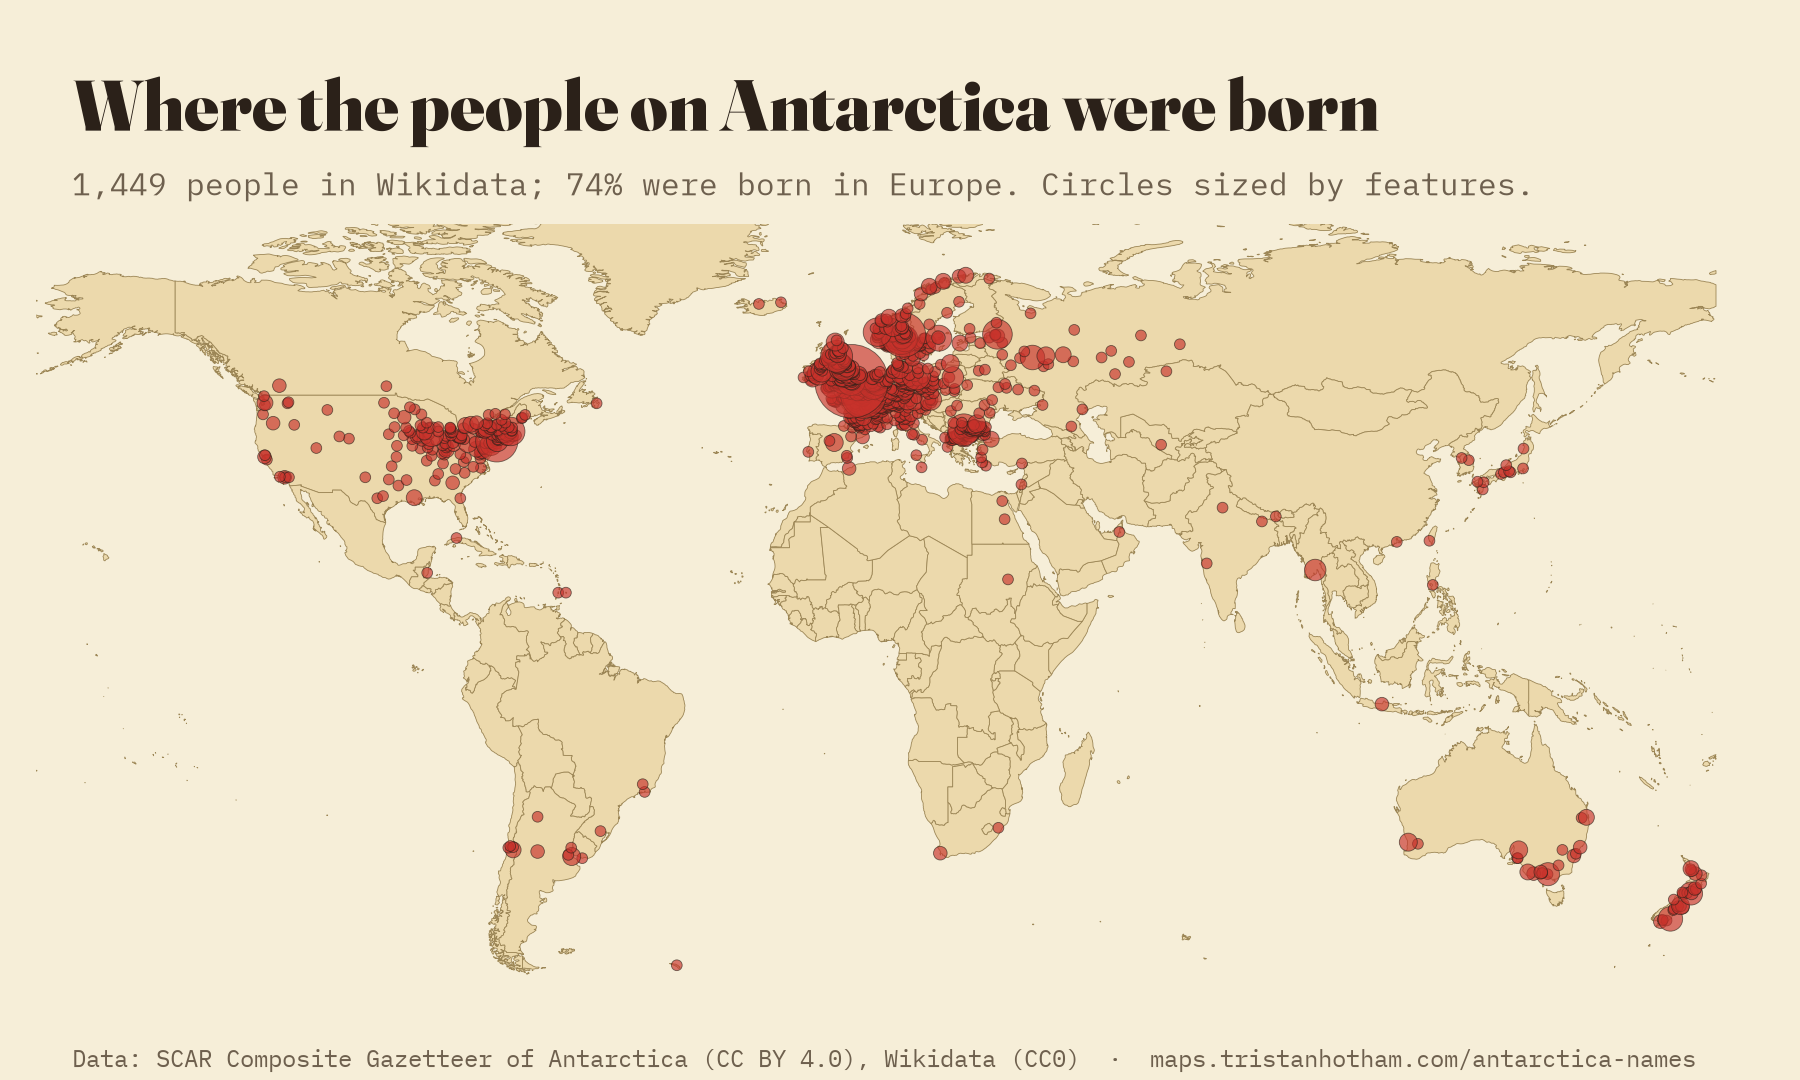
\includegraphics[width=0.9\textwidth]{f_birthplaces.png}
\caption{Birthplaces of the people honoured, from Wikidata. Circle area: number of features.}\label{fig:birth}\end{figure}

\subsection{Different names for the same feature}
1,038 features (8.7\% of those in more than one gazetteer) carry names that differ by more than spelling or transliteration. Some are translations (Seal Nunataks, Robbeninseln, nunataks Foca); many are distinct names, concentrated on the Antarctic Peninsula: 661 involve the Argentine gazetteer and 574 the Chilean one. Admiralty Bay, for example, is the Bah\'ia Almirantazgo in Chile's list and the bah\'ia Lasserre in Argentina's.

\section{Limitations}
First, the narratives are uneven: the American, British, Australian and New Zealand ones are full, while many Russian, Argentine and Chinese entries have no narrative or none in English, so 18.8\% of features have no recorded meaning and the shares by nation rest on different bases. Second, the rules misread a minority of narratives; audits suggest about 90 to 95\% are read correctly, with errors biased towards ``other'' and ``not stated'', so the share of people is if anything understated. Third, the naming nation is weakest where it rests on approval dates (956 features). Fourth, naming years are often approval years. Fifth, Wikidata covers only some of the people honoured, and its birthplaces carry their own errors. Sixth, the claims are drawn as sectors to 60$^\circ$S; their exact limits are not all defined. Undersea features (254, those in SCAR's sea-floor class or only in the GEBCO undersea list) are counted as features but left out of every claim share, and the 59 features of Peter I Island, a Norwegian dependency at 90.6$^\circ$W, count with Norway's claim rather than with unclaimed Marie Byrd Land. Seventh, where the narrative does not name the namer, the expedition that discovered or charted a feature stands in for the namer (1,559 features), which can credit a name to the nation that first photographed a feature rather than the one that named it.

\section{Conclusion}
Antarctica's map is a record of who was there and who paid, in the second half of the twentieth century. The United States and Britain named nearly half of it; claimant states named mostly inside their claims but not most of what they claim; the busiest decades followed the IGY; and the people honoured are overwhelmingly European-born men, many of them the scientists, airmen and cooks of national programmes. Bulgaria's recent naming of the Peninsula after its own towns shows that the process is still going on. Reading the narratives at scale makes these patterns measurable, and the published feature table lets anyone check a name.

\section*{Data and code availability}
The interactive map is at \url{https://maps.tristanhotham.com/antarctica-names/}. Data and code are at \url{https://github.com/Tristan-Hotham/antarctica-names} and archived with this paper at https://doi.org/10.5281/zenodo.24075309. Derived data and text are released under CC BY 4.0, as is the SCAR gazetteer they derive from (Wikidata is CC0); code under the MIT licence.

\section*{AI statement}
I wrote the text, with drafting and editing assistance from Claude (Anthropic), which also helped prepare the analysis code. I reviewed and checked all text and results.

\begin{thebibliography}{9}
\bibitem[Alberts(1995)]{alberts} Alberts, F. G. (ed.) (1995) \textit{Geographic Names of the Antarctic}, 2nd edition. United States Board on Geographic Names; National Science Foundation, Arlington, VA.
\bibitem[Antarctic Treaty(1959)]{treaty} The Antarctic Treaty (1959). Signed at Washington, 1 December 1959. \textit{United Nations Treaty Series} 402, 71.
\bibitem[Bast and Buchhold(2017)]{qlever} Bast, H. and Buchhold, B. (2017) QLever: a query engine for efficient SPARQL+Text search. In \textit{Proceedings of the 2017 ACM Conference on Information and Knowledge Management (CIKM 2017)}, 647 to 656. ACM.
\bibitem[Natural Earth(2026)]{naturalearth} Natural Earth (2026) Admin 0 countries 1:10m and 1:50m, land 1:50m, populated places. Public domain. \url{https://www.naturalearthdata.com/}
\bibitem[OpenStreetMap contributors(2026)]{osm} OpenStreetMap contributors (2026) OpenStreetMap, served as OpenMapTiles vector tiles by OpenFreeMap. ODbL.
\bibitem[Secretariat SCAR(1992)]{scar} Secretariat SCAR (1992, updated 2014) \textit{Composite Gazetteer of Antarctica}. Scientific Committee on Antarctic Research. GCMD metadata \url{http://gcmd.nasa.gov/records/SCAR_Gazetteer.html}; data served by the Australian Antarctic Data Centre, CC BY 4.0, accessed 2026.
\bibitem[Stewart(2011)]{stewart} Stewart, J. (2011) \textit{Antarctica: An Encyclopedia}, 2nd edition. McFarland, Jefferson, NC.
\bibitem[Vrande\v{c}i\'c and Kr\"otzsch(2014)]{wikidata} Vrande\v{c}i\'c, D. and Kr\"otzsch, M. (2014) Wikidata: a free collaborative knowledgebase. \textit{Communications of the ACM} 57(10), 78 to 85. \url{https://doi.org/10.1145/2629489}
\end{thebibliography}
\end{document}
